\chapter{Configurar RAID 1 durante la instalación de Ubuntu}

Tal como hemos podido ver anteriormente, durante la \hyperlink{instalar_ubuntu_lts}{instalación de Ubuntu 20.04}, en el paso 7 podemos realizar la instalación en el disco duro que tengamos instalado en el servidor físico o en la máquina virtual.

En este paso podemos realizar distintas configuraciones:

\begin{center}
    \vspace{-15pt}
    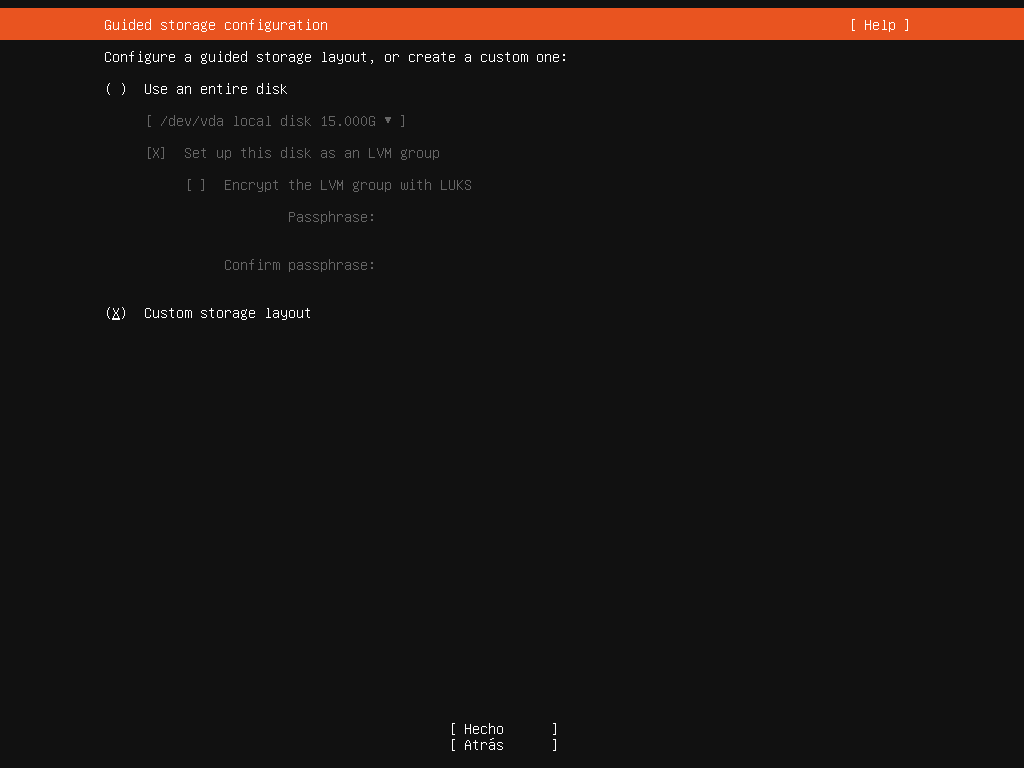
\includegraphics[width=10cm]{01_storage_layout.png}
    \vspace{-10pt}
\end{center}

\begin{itemize}
    \item Usar el disco entero.
    \begin{itemize}
        \item Nos permitirá crear un sistema con LVM (por defecto activado) y con posibilidad de cifrar la partición creada.
    \end{itemize}
    \item Crear un diseño de almacenamiento personalizado.
\end{itemize}

    En la segunda opción podremos:
\begin{itemize}
    \item  Crear particiones a nuestro gusto.
    \item  Elegir el sistema de ficheros de las particiones.
    \item  Crear sistema RAID por software.
\end{itemize}


\section{Pasos previos}
Dado que vamos a crear un sistema RAID 1 durante la instalación de Ubuntu, necesitaremos al menos \textbf{dos discos duros} en nuestro servidor antes de comenzar con la instalación.

En nuestro sistema virtualizado hemos añadido dos discos duros de igual tamaño (15GB), en los cuales crearemos particiones para posteriormente sobre ellas realizar el RAID 1.

\section{Entendiendo las particiones a realizar}
En este apartado vamos a explicar la teoría que está detrás del sistema de particionado que vamos a necesitar crear y que posteriormente realizaremos en el sistema de instalación de Ubuntu.

\subsection{Situación inicial: discos duros sin particionar}
Como ya se ha comentado, en nuestro servidor vamos a contar con dos discos duros de igual tamaño. Esto suele ser lo habitual, pero lo importante es que las particiones que vayamos a crear sean del tamaño exacto, aunque un disco duro sea de mayor tamaño (aunque lógicamente, ese espacio quedará desaprovechado).

En la siguiente imagen vemos que tenemos dos discos duros de 15GB de tamaño cada uno:

\begin{center}
    \vspace{-10pt}
    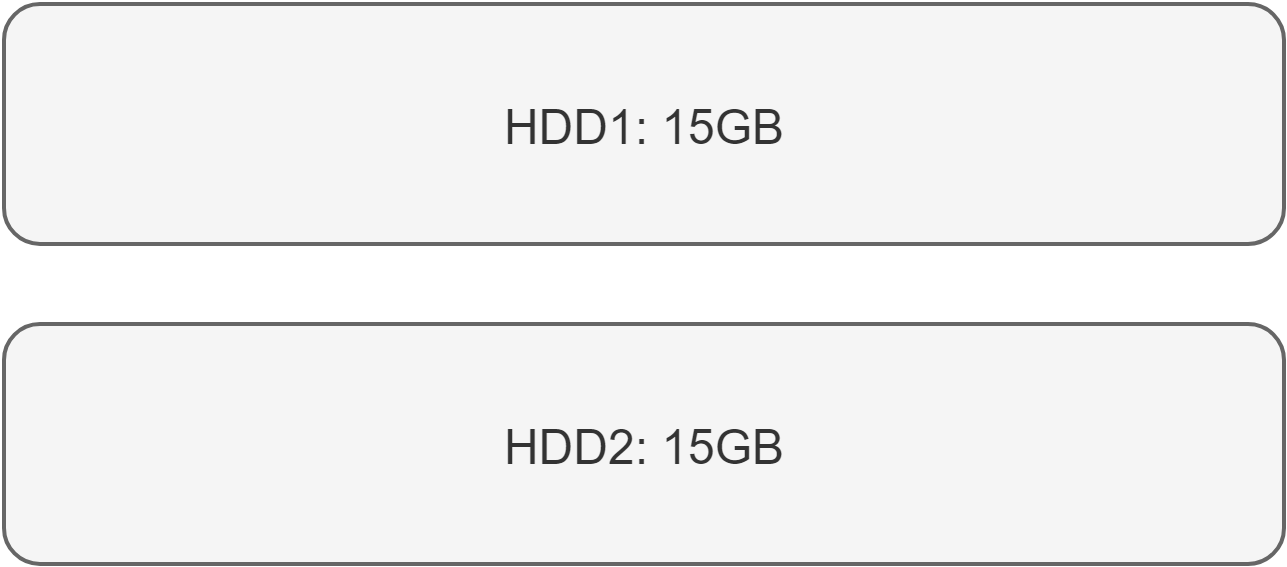
\includegraphics[width=8cm]{raid1_01.png}
    \vspace{-20pt}
\end{center}


\subsection{Particionado inicial}
A continuación vamos a tener que pensar cómo van a ser las particiones que vamos a necesitar en nuestro servidor. En nuestro caso vamos a crear dos:
\begin{itemize}
    \item  \textbf{14GB}: Sistema operativo.
    \item  \textbf{1GB}: (o hasta completar) SWAP.
\end{itemize}

Como se puede entender, al tener una única partición, todo el sistema raiz “/” va a ir en ella, mientras que la otra partición será la usada para el área de intercambio.

Es importante entender que en este paso sólo \textbf{vamos a crear las particiones pero sin darles formato}. Por lo tanto, nuestros discos duros ahora tendrían este aspecto:

\begin{center}
    \vspace{-10pt}
    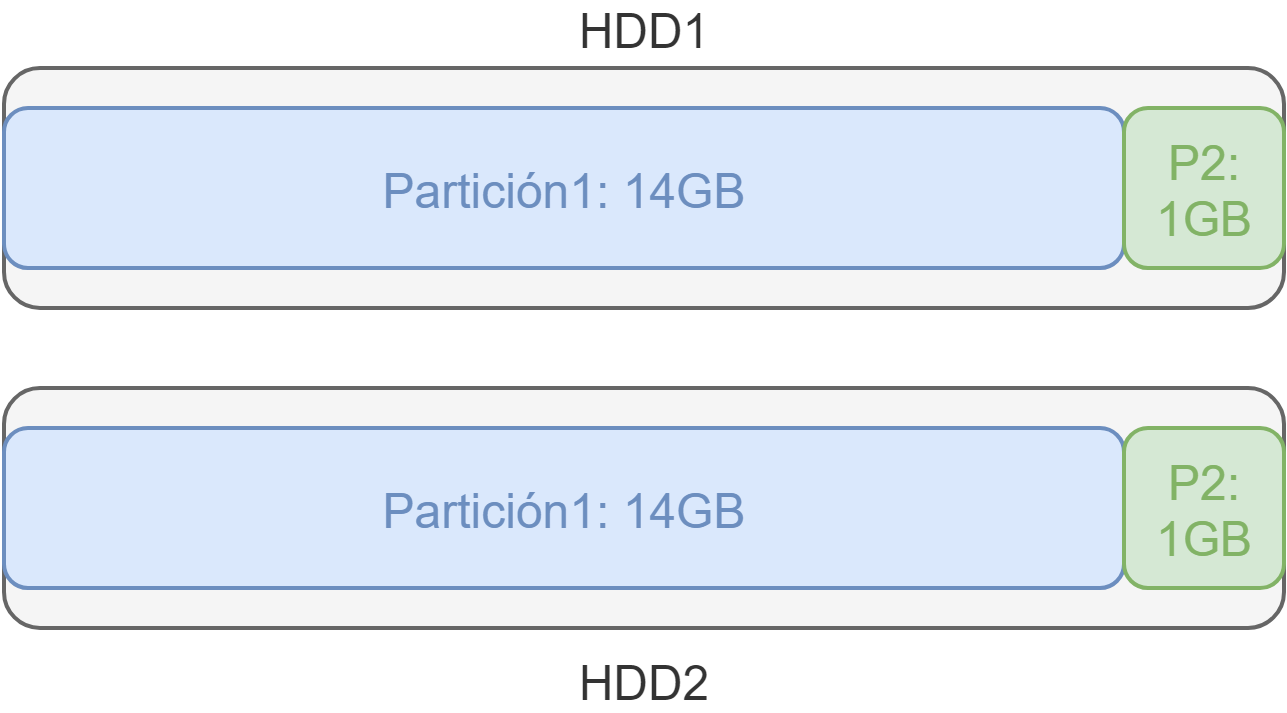
\includegraphics[width=8cm]{raid1_02.png}
    \vspace{-20pt}
\end{center}



\subsection{Crear particiones RAID}
El siguiente paso es crear las particiones “virtuales” RAID. Vamos a crear una primera partición RAID que va a incluir las particiones de 14GB de ambos discos duros, y la segunda partición virtual incluirá las particiones de 1GB.

\begin{center}
    \vspace{-10pt}
    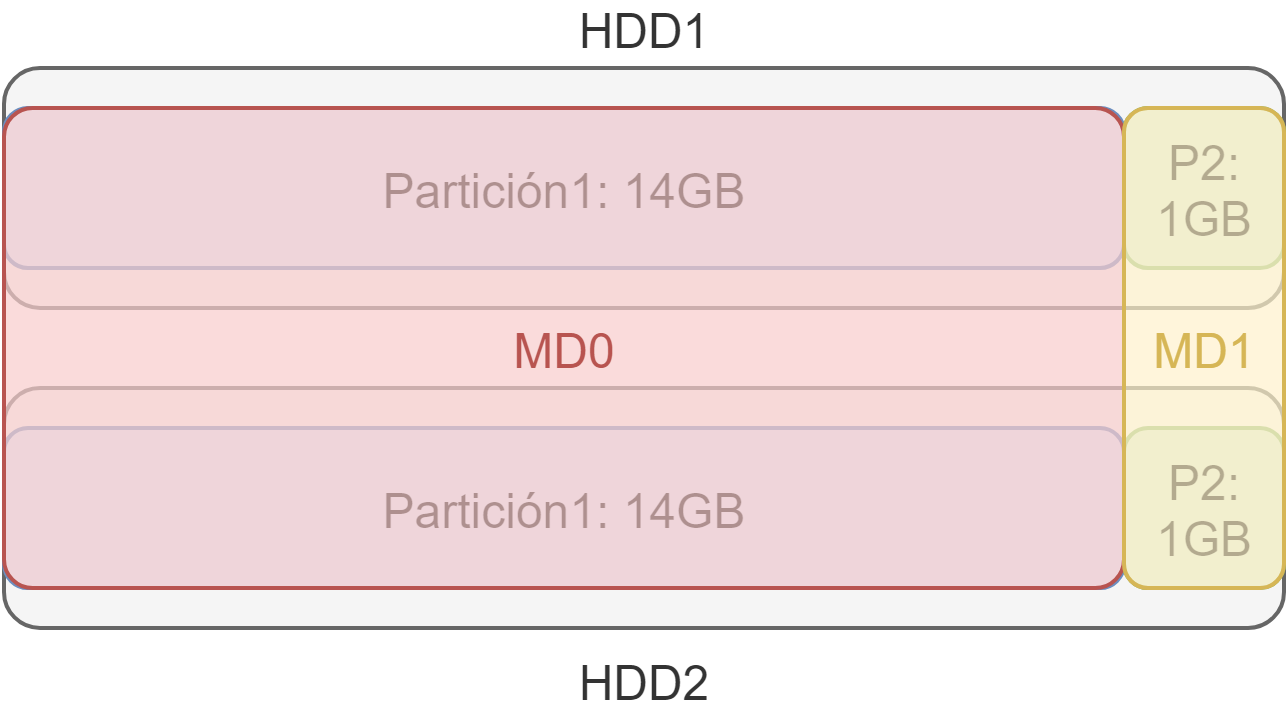
\includegraphics[width=8cm]{raid1_03.png}
    \vspace{-20pt}
\end{center}

De esta manera, tendremos unas particiones MD0 y MD1 que son particiones virtuales.

\subsection{Formatear particiones RAID con el formato adecuado}
El último paso de la instalación es hacer uso de las particiones RAID creadas y formatearlas con el sistema de ficheros acorde a las necesidades que tengamos, y elegir el punto de montaje adecuado.

\begin{center}
    \vspace{-10pt}
    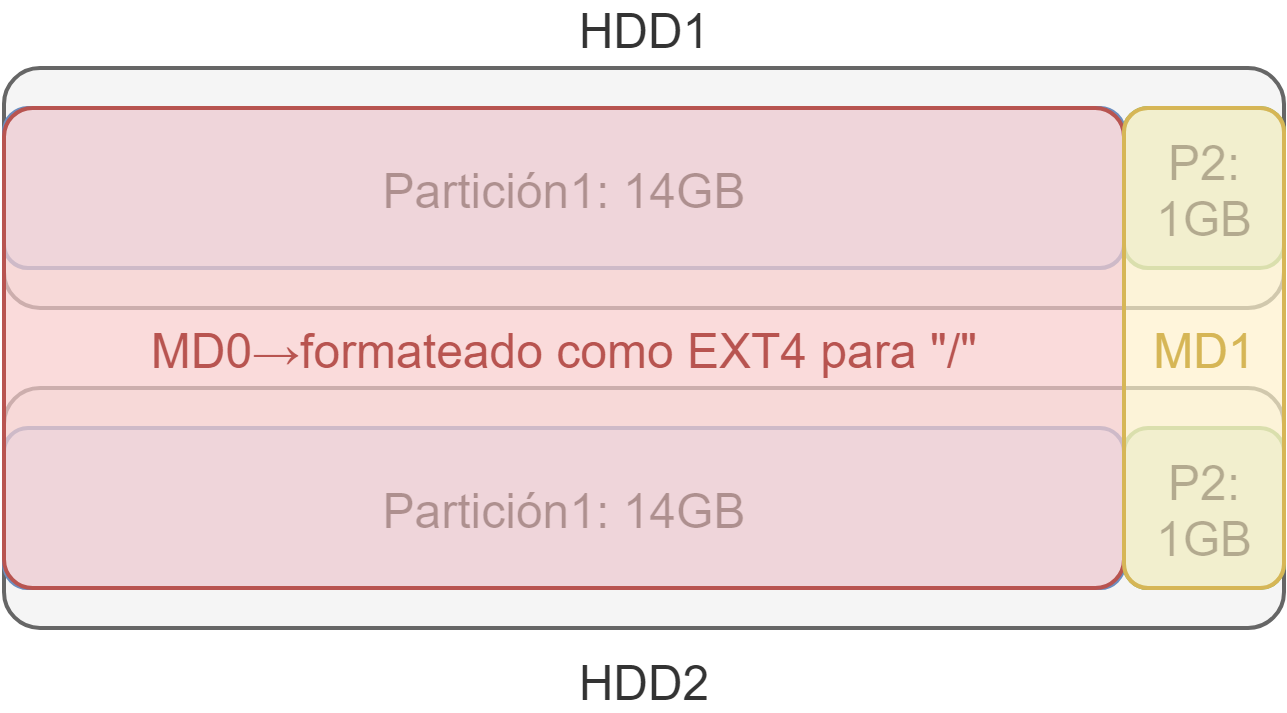
\includegraphics[width=8cm]{raid1_04.png}
    \vspace{-20pt}
\end{center}

En nuestro caso va a ser:
\begin{itemize}
    \item  \textbf{MD0}: sistema de ficheros ext4 y lo vamos a utilizar como sistema de ficheros raíz “/”.
    \item  \textbf{MD1}: formateado como SWAP y actuará como área de intercambio.
\end{itemize}

Tras este paso, la instalación del sistema operativo puede continuar de la manera habitual.

\section{Realizando el particionado en el instalador de Ubuntu}
Tras haber entendido las particiones que vamos a realizar, ahora es el momento de proceder en el instalador de Ubuntu. Vamos a seguir los mismos pasos que hemos explicado en el apartado anterior, de esta manera aplicaremos lo aprendido a nivel teórico.

\subsection{Situación inicial: discos duros sin particionar}
Tal como hemos comentado previamente, en el paso 7 de la instalación, elegiremos la opción de crear un “diseño de almacenamiento personalizado”. Tras entrar en esta opción, el instalador tendrá el siguiente aspecto:

\begin{center}
    \vspace{-10pt}
    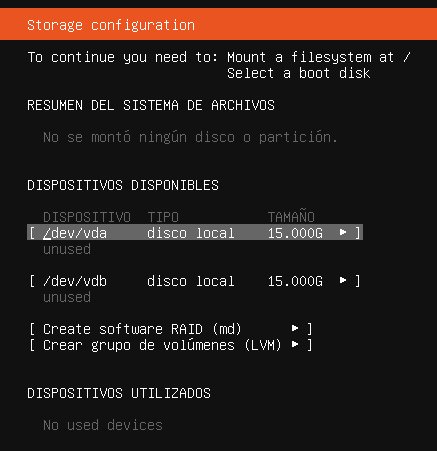
\includegraphics[width=8cm]{ubuntu_raid1_01.png}
    \vspace{-20pt}
\end{center}

Tal como se puede ver, tenemos dos discos duros en el sistema: \textbf{vda} y \textbf{vdb}. El nombre de los discos viene de \textbf{V}irtual \textbf{D}isk, dado que la instalación la estamos realizando en una máquina virtual.

\subsection{Particionado inicial}
En este paso vamos a crear en cada uno de ellos la partición de 14GB y  el resto del espacio la usaremos para la segunda partición.

\subsubsection{Marcar discos como dispositivos de arranque}
Por cómo funciona el sistema de arranque de Linux, antes de realizar las particiones vamos a marcar que ambos discos duros sean dispositivos de arranque (“Boot Device”). Para ello pulsaremos “Intro” en cada uno de los discos y elegiremos la opción correspondiente (imágenes de cada disco):

\begin{center}
    \vspace{-10pt}
    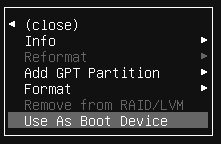
\includegraphics[width=4cm]{ubuntu_raid1_02-1.png}
    \hspace{3cm}
    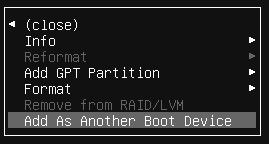
\includegraphics[width=4.90cm]{ubuntu_raid1_02-2.png}
    \vspace{-20pt}
\end{center}

De esta manera, el instalador de Ubuntu creará una pequeña partición al inicio del disco donde al terminar se realizará la instalación del sistema de arranque GRUB en ambos discos duros.


\subsubsection{Crear particiones}
Ahora es el momento de crear las particiones, y los pasos serán seleccionar el disco duro, pulsar “Intro”, se nos desplegará un pequeño menú y vamos a elegir la opción  \textit{“Add GPT Partition”} y rellenaremos el tamaño de la partición que nos interese en el momento y el formato lo dejaremos en \textit{“Leave unformatted”} (dejar sin formatear).

\begin{center}
    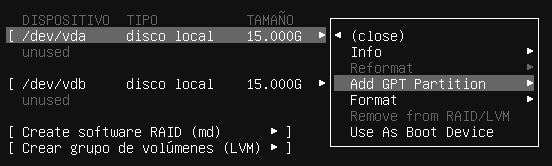
\includegraphics[width=8cm]{ubuntu_raid1_03.png}
    \hfill
    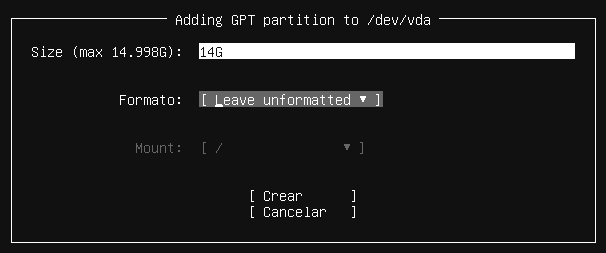
\includegraphics[width=8cm]{ubuntu_raid1_04.png}
\end{center}

Estos pasos lo realizaremos en cada disco duro con las particiones que vamos a necesitar, quedando al finalizar el sistema así:

\begin{center}
    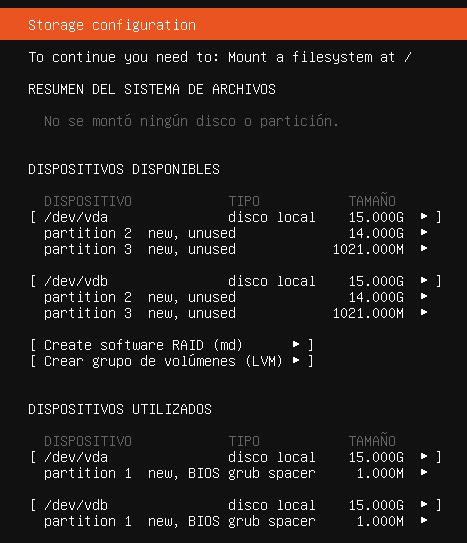
\includegraphics[width=8cm]{ubuntu_raid1_05.png}
\end{center}

Tal como se puede ver, cada disco duro tiene dos particiones con el tamaño deseado que no están siendo utilizadas, y en la parte de abajo aparecen las particiones denominadas “BIOS grub spacer”.


\subsection{Crear particiones RAID}
El siguiente paso es crear las particiones RAID en las que haremos que el sistema cree un RAID 1 haciendo uso de las particiones de los discos duros físicos. Seleccionaremos la opción “\textit{Create software RAID (md)}” y nos aparecerá una ventana en la que podremos elegir:

{
    \begin{minipage}{9cm}
        \begin{itemize}
            \item \textbf{Nombre}: de la partición que vamos a crear. Es habitual que estas particiones empiecen por “\textbf{md}”, ya que viene de “\textit{multiple device}”.
            \item \textbf{Nivel RAID}: Podremos elegir entre las versiones 0, 1, 5, 6 y 10 de RAID. Por defecto está seleccionada la opción RAID 1.
            \item  \textbf{Dispositivos}: sobre el que aplicaremos el RAID.
        \end{itemize}
    \end{minipage}
    \hfill
    \begin{minipage}{7cm}
        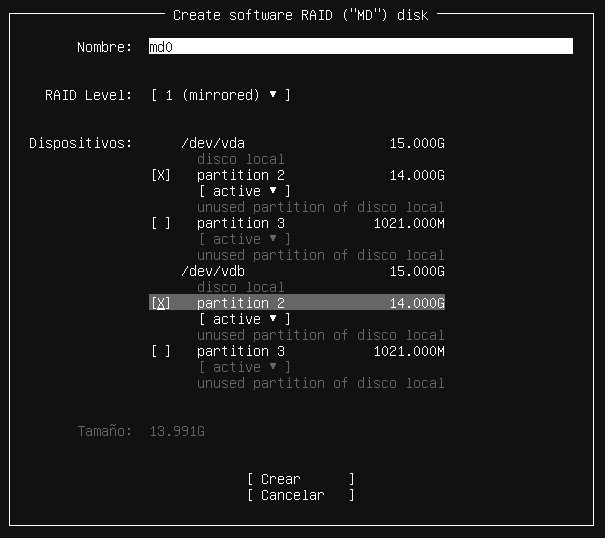
\includegraphics[width=7cm]{ubuntu_raid1_06.png}
    \end{minipage}
}


Crearemos primero \textbf{md0} seleccionando las particiones de 14GB tal como aparece en la siguiente imagen:

Y a continuación crearemos \textbf{md1} con las particiones restantes. Tal como se puede ver a continuación, las particiones de 14GB ya no aparecen, porque están siendo usadas en el otro RAID.

\begin{center}
    \vspace{-10pt}
    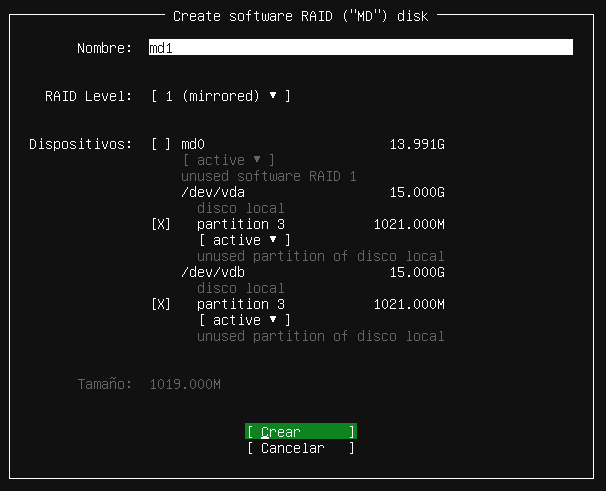
\includegraphics[width=9cm]{ubuntu_raid1_07.png}
    \vspace{-20pt}
\end{center}


Tras la creación de los dispositivos “md”, nos aparecerán como dispositivos disponibles para usarlas en el siguiente paso:

\begin{center}
    \vspace{-10pt}
    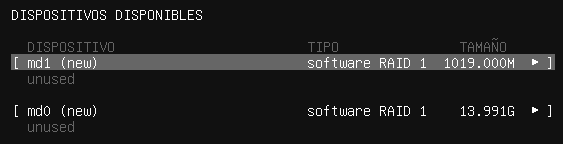
\includegraphics[width=9cm]{ubuntu_raid1_08.png}
    \vspace{-20pt}
\end{center}

\subsection{Formatear particiones RAID con el formato adecuado}
Aunque este paso lo vamos a realizar sobre las particiones RAID creadas previamente, es un paso que es habitual realizar cuando queremos que nuestra instalación tenga un sistema de particiones propio.

Tenemos que pensar que las particiones RAID ahora son como particiones normales, a las que les vamos a querer dar un formato y utilizarlas para realizar la instalación.

Vamos a seleccionar la primera, \textbf{md0}, posicionándonos encima de ella y dándole a “Intro” y posteriormente dándole a “\textit{Add GPT partition}”:

\begin{center}
    \vspace{-10pt}
    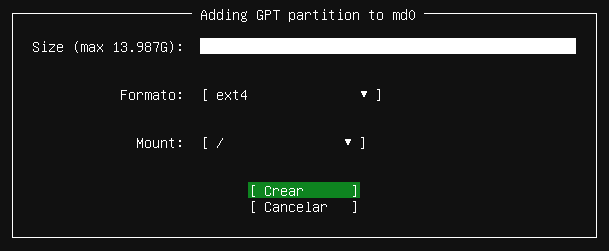
\includegraphics[width=8cm]{ubuntu_raid1_09.png}
    \vspace{-20pt}
\end{center}

Dejaremos el tamaño en blanco, indicando que usaremos todo el espacio libre, lo vamos a formatear con el sistema de ficheros \textbf{ext4} y se va a montar como el sistema de ficheros “/”.

En \textbf{md1} también le daremos a crear nueva partición, y haremos lo mismo pero usando el formato \textbf{swap}. Quedando una vez terminado el sistema de particiones de la siguiente manera:

\begin{center}
    \vspace{-10pt}
    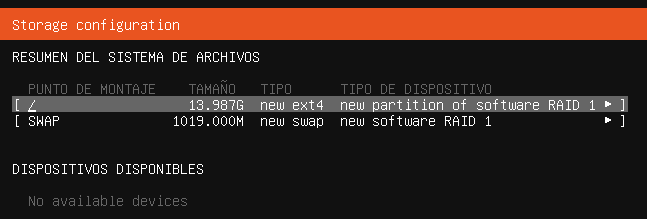
\includegraphics[width=8cm]{ubuntu_raid1_10.png}
    \vspace{-20pt}
\end{center}

Y tras esto podremos continuar la instalación de manera normal.
\clearpage